

%\documentclass{scrippsthesis}
\documentclass[a4paper,11pt,twoside]{UUthesis}
%\usepackage[pass]{geometry}
%%% HEADER INFORMATION %%%

\title{Title}
\author{Julia Ruiter}
%\reader{Chris Towse}
%\reader{Adam Landsberg}

%%% Including new commands and packages.

% Allows for auto formatting of theorems,
% definitions etc.
\usepackage{amsthm}
\usepackage{graphics,graphicx}
\usepackage{tikz}
\usepackage{verbatimbox}
\usepackage{textgreek}
\usepackage[toc,page]{appendix}
\usepackage{float}
\usepackage{amsmath}


\newtheorem{thm}{Theorem}[chapter]
\newtheorem{lem}[thm]{Lemma}
\newtheorem{prop}[thm]{Proposition}
\newtheorem{cor}[thm]{Corollary}

\theoremstyle{definition}
\newtheorem{defn}[thm]{Definition}
\newtheorem{ex}[thm]{Example}

\theoremstyle{remark}
\newtheorem*{rmk}{Remark}
\newtheorem*{notn}{Notation}
\newtheorem*{pf}{Proof}

% Add any new commands here.
\newcommand{\Q}{\mathbb{Q}}
\newcommand{\Z}{\mathbb{Z}}
\newcommand{\F}{\mathbb{F}}
\newcommand{\R}{\mathbb{R}}
\newcommand{\NN}{\mathbb{N}}

%file path for images


%%%  END HEADER %%%

\begin{document}
%\begin{comment}

\frontmatter

\maketitle % Title page
%
%
%%%% ABSTRACT.
%
\begin{abstract} 
[write text here]]
\end{abstract}

%%% CONTENTS, FIGURES, TABLES
\tableofcontents
\listoffigures
%\listoftables

%%% ACKNOWLEDGEMENTS.

%\begin{acknowledgments}
%...(write here later)
%\end{acknowledgments}

%%% End of the front matter.

%% MAIN MATTER - INCLUDE THE CHAPTERS.
\mainmatter

% CHAPTERS %

\chapter{Lorenz, Liu, and Other Chaotic Systems}

\par Thanks to $\it{Jurassic Park}$, most everyone is familiar with the idea of the ``Butterfly Effect'':  the idea that one small perturbation in the present can set the future on a wildly different course.  This idea comes from Ed Lorenz, chaos theory's pioneer, and his observations of dynamical systems with strange attractors, that is, systems of equations that have an element of chaos built into them.  These systems are a part of the family of Lorenz equations and are of the following form:
%
\begin{equation}
\begin{cases} 
\dot{x} = \sigma(y-x) \\ 
\dot{y} = rx - y - xz \\ 
\dot{z} = xy - bz
\end{cases}
\end{equation}
%
%Figure \ref{fig:genLorenz} original Lorenz system
%  use math mosde $_$ for all variables in paragraphs
where the dot denotes the first time derivative of each variable, and with the Prandtl number ($\sigma$), Rayleigh number($r$), and $b$ all greater than 0.  The aperiodic nature of this system defined by a total lack of fixed points and quasiperiodic orbits for any initial trajectory means that the outcome is very sensitive to its initial conditions.  The deterministic nature of the system, the fact that its irregularity comes not from randomness, but the nonlinear relationships of variables, means that once the initial conditions have been set, the outcome at any given time $t_0$ is always going to give the same values $x$, $y$, $z$.  These two attributes make the Lorenz equations a very good candidate for an encryption system (more on that in the next chapter).  

\begin{figure}[H]
    \centering
	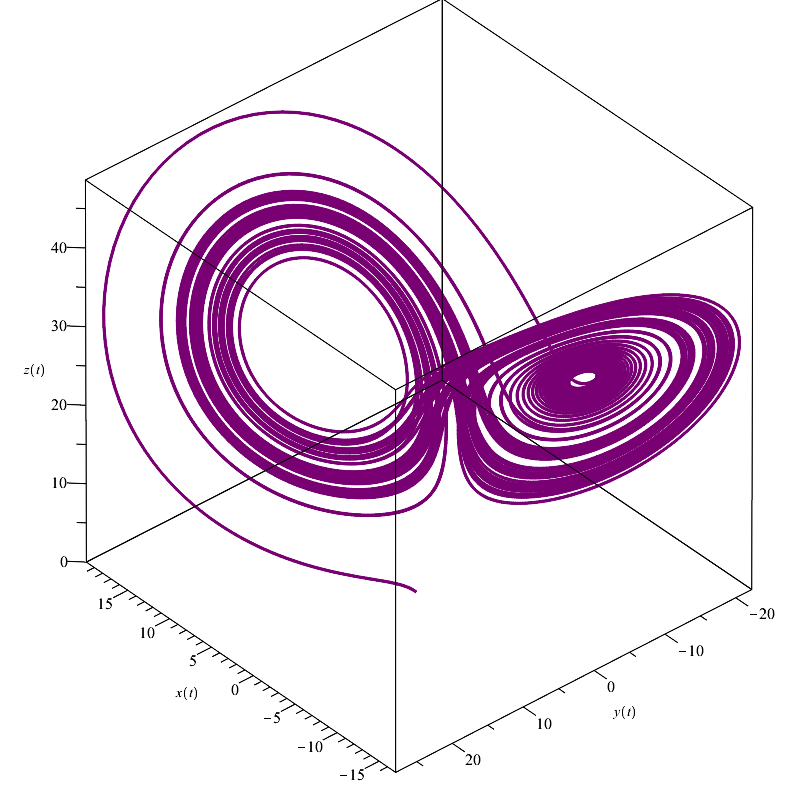
\includegraphics[width=\linewidth]{Figures/lorenz2.PNG}
	\caption{Lorenz System where $r = 28, \sigma = 10, and b = 8/3$. *}
	\label{fig:genLorenz}
\end{figure}

\par In other words, chaotic systems have a dense orbit, meaning that the system has at least two orbits that are sensitive to the initial conditions, thus excluding systems with only one cycle as well as systems consisting of just an equilibrium point which are systems with clear orbits in their phase space (to be defined in glossary). 

\par The most notable feature of the Lorenz systems is that it contains a strange attractor.  An attractor is a subset A of the system's phase space where the neighborhood of A is defined as being the basin of attraction, the basin of attraction being the region of phase space where the system starts to show cyclic action, usually resulting in a stable orbit, or condensing towards a point.  Strange attractor differ, however, in that given any two points arbitrarily close to each other in one orbit, several orbits later will be arbitrarily further away, rather than same or closer.  It is this quality that makes the system chaotic.

\par What is important to note, though, is that not all values of $r$, $b$, and $\sigma$ will yield a chaotic system. An analysis of the bifurcation diagrams (a diagram that shows values for which there are stable and unstable equillibria) of $r$ help explain why only certain values work.

\par for Lorenz systems, there is always an equilibrium at the origin $(0,0,0)$, this is true of any variation of the Lorenz system, using any values $b$, $r$, and $\sigma$.  However, if $r>1$, then other critical points appear:
%
\begin{equation}
(\sqrt{b(r-1)},\sqrt{b(p-1)},(r-1))
\end{equation}
\begin{equation}
(-\sqrt{b(r-1)},-\sqrt{b(p-1)},(r-1))
\end{equation}
%
which means the system exhibit cyclical behaviour if and only if $r$ and $\sigma$ are positive and have the property that:
%
\begin{equation}
\sigma > b + 1 
\end{equation}
\begin{equation}
r > \sigma \frac{\sigma + b + 3}{\sigma - b - 1}
\end{equation}
%
because of that, the original version of the Lorenz system (and the one used later in this text) is usually restricted to values close to:
\begin{equation}
\begin{cases} 
r = 28 \\ 
b = \frac{8}{3} \\ 
\sigma = 10
\end{cases}
\end{equation}
%
which are the original set of values that Lorenz accidentally discovered that exhibited chaotic behaviour.

\par What happens if the variables don't all fall in this range?  Take this example where only the value of \textsigma has been altered:
%
\begin{figure}[H]
    \centering
	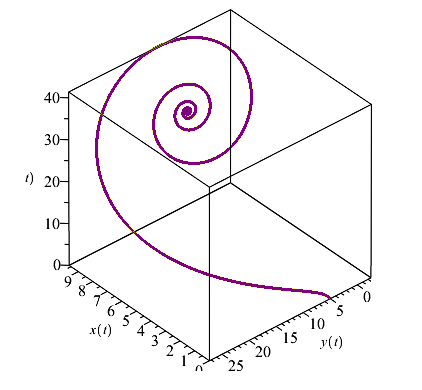
\includegraphics[width=\linewidth]{Figures/lorenz_s2.png}
	\caption{Lorenz System where $r = 28, \sigma = 1, and b = 8/3$}
	\label{fig:badLorenz}
\end{figure}
%Figure \ref{fig:badLorenz} nonchaotic Lorenz system
%
As you can see, the resulting graph is not at all chaotic, with x, y, and z all having a fixed limit (regular attractor) as time goes to infinity, or otherwise exhibiting standard actions as dynamical system.  This means that distance between two points at t0 will always be larger than the distance between those points at a later $t_1$, meaning that it is easy to predict how the system behaves over time.  Because of the predictability, a Lorenz system with these parameters cannot be used to encrypt information, as values follow a predictable pattern.  For that reason, we will only consider Lorenz systems with chaotic action (like those mentioned at the beginning of the chapter) as candidates for strong encryption.

%
\subsection{Liu and Chen Systems}

\par Lorenz systems are not the only type of dynamical system that exhibit this sort of chaotic behaviour.  Two other systems, Liu and Chen, are variations of the Lorenz system, with slightly different dependencies and thus different usable chaotic parameters.

\par Although it is a bit difficult to see, the Chen and Liu systems actually shows greater levels of chaos that the Lorenz system, and thus are better candidates for chaotic encryption.  Because of this, these systems, though only discovered in the past 15 years,  are most often used and referenced in current publications in this field.

\par Take the Chen system:
%
\begin{equation}
\begin{cases} 
\dot{x} = a(y - x) \\ 
\dot{y} = (c - a)x + cy + xz \\
\dot{z} = xy - bz
\end{cases}
\end{equation}
%
\par 

%


%\end{equation}
% backslash square bracket to start equation
% \cite to cite in text
% tex will not display sources that are not refrenced ==> FIXED with nocite


%\end{comment}


%%% End of the main matter.
\backmatter

%%%% BIBLIOGRAPHY (Be sure cto compile with BibTeX to make this work!)
%
\nocite{*} % Show everything in bib file, not just things that are explicitly cited.
\bibliography{bibliography}
\bibliographystyle{alpha}
%\printbibliography


\end{document}

% double check/cross with original doc--might be undoing what is going on in 
% have to bibtex bibliography first, then can tex rest of file